\question[5] Considera los dos triángulos que se muestran abajo en la Figura \ref{fig:20230323153911} (los triángulos no están dibujados a escala).

\begin{figure}[H]
    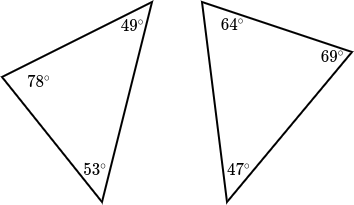
\includegraphics[width=0.5\linewidth]{../images/20230323153911}
    \caption{}
    \label{fig:20230323153911}
\end{figure}

\textbf{¿Los dos triángulos son congruentes?}
\emph{Escoge 1 respuesta:}

\begin{choices}
    \choice Sí.
    \CorrectChoice No.
    \choice No hay suficiente información para decidir.
\end{choices}

\begin{solutionbox}{5cm}
    Dos triángulos son congruentes si tienen la misma forma y tamaño. En otras palabras, dos triángulos son congruentes si todos los lados y ángulos correspondientes son congruentes.

    En este caso, ya conocemos los tres ángulos en ambos triángulos y no hay dos que sean iguales.
    Por lo tanto, es imposible que los ángulos correspondientes sean congruentes y entonces los triángulos no son congruentes.

    No, los triángulos no son congruentes.
\end{solutionbox}